% Provenance (never printed): see sources/outline_sources.md (Year 2: energy geology --- the
% petroleum system quantified, unconventional resources, geothermal systems, uranium deposits,
% geological storage of carbon dioxide).
% Kerogen kinetics and elemental analyses: Fletcher and Pugmire (DOE, OSTI 1176871); kerogen
% types and Easy%Ro: Advanced Chemistry Basins Project (DOE, OSTI 830009); maturity thresholds:
% USGS MF-2008-B; TTI: Waples (1980) and Hammerschmidt et al. (2014); volumetrics and CO2
% storage: DOE/NETL (2008) and IPCC SRCCS (2005) chapter 5; geothermal: USGS OFR 2008-1296 and
% FS 2008-3082; uranium: USGS Bulletin 1693; Oklo: OSTI abstract records. Ledger rows in
% sources/ledger/book4.md; curves from figdata/bachelor-2/maturation.py and co2_density.py,
% numbers from the Book 4 second-writer scratch calculator calc/ch30.py.
% Geology and sourced numbers only: no advocacy, no policy.
\chapter{Energiegeologie}\label{ch:b2:energy-geology}

Olie is de rest van microscopische organismen, begraven met modder en miljoenen jaren gekookt bij
ongeveer \qty{100}{\celsius}; geothermische energie is diezelfde warmte van de aarde, rechtstreeks gewonnen.
Beide worden beheerst door temperatuur en tijd: de eerste door de snelheid waarmee een chemische reactie verloopt terwijl
begraven gesteenten langzaam opwarmen, de tweede door hoeveel warmte een volume gesteente opslaat en hoe snel water
die naar een put kan voeren. Dit hoofdstuk kwantificeert het petroleumsysteem, gaat dan over naar de voorraden waaraan
een van zijn elementen ontbreekt, naar geothermische warmte en naar uranium, en eindigt met de omgekeerde operatie:
koolstofdioxide terug onder de grond brengen.
% ledger: earle:oil-window, earle:organic-preservation

\begin{recall}
\textbf{Uit de schoolboeken}: brongesteente, kerogeen, rijping, olievenster, migratie,
reservoirgesteente, afdekgesteente, val, dekpakket, petroleumsysteem; steenkool en inkolingsgraad; geothermische energie.
\textbf{Uit Boek~3}: warmtestroom en de geotherm; porositeit en permeabiliteit;
poriënvloeistofdruk, effectieve spanning en het criterium van Coulomb; boorstaat; sedimentair bekken en
subsidentie. \textbf{Uit de scheikundeboeken}: de wet van Arrhenius, activeringsenergie,
eerste-ordereactie. \textbf{Uit de natuurkundeboeken}: radioactief verval, vervalconstante, halveringstijd; het
kritieke punt van een fluïdum. \textbf{Uit \cref{ch:b2:basins-compared}}: \omterm{def:b2:basins-compared:curve}{subsidentiecurve}.
\textbf{Uit \cref{ch:b2:ore-deposits}}: \omterm{def:b2:ore-deposits:types}{ertsafzettingstype}, \omterm{def:b2:ore-deposits:grade}{tonnage}.
\end{recall}

\section{Het petroleumsysteem gekwantificeerd}\label{sec:b2:energy-geology:petroleum}

Een petroleumsysteem vraagt een brongesteente rijk aan kerogeen, een reservoir, een afdekgesteente, een val en genoeg
dekpakket om het brongesteente te verhitten, en de gebeurtenissen moeten in de juiste volgorde komen: de val moet
bestaan wanneer de olie migreert. Het kwantificeren betekent drie vragen beantwoorden: welk soort kerogeen
het brongesteente bevat, hoe ver het is omgezet, en hoeveel van het product in de
val zit.
% ledger: magoon00:tps

\begin{definition}[Kerogeentype, van Krevelen-diagram]\label{def:b2:energy-geology:kerogen}
Kerogenen vallen naar hun elementsamenstelling uiteen in drie \emph{kerogeentypen}\index{kerogeentype}:
type~I, sapropelisch, het rijkst aan waterstof, dat vooral olie levert; type~III, humisch of steenkoolachtig,
arm aan waterstof, dat vooral methaan levert; en type~II, intermediair, een bron van zowel olie
als gas. Het \emph{van Krevelen-diagram}\index{van Krevelen-diagram} zet de atomaire verhouding H/C van
een kerogeen uit tegen zijn atomaire verhouding O/C; de typen nemen er verschillende gebieden in, en de rijping
verplaatst een kerogeen naar lage H/C en lage O/C.
\end{definition}

Zeven onrijpe kerogenen van bekend type, geanalyseerd in één laboratoriumstudie, hebben een atomaire H/C van
1.51 en 1.61 (type~I, waaronder de Green River-olieschalie van Utah, afgezet in meren en rijk aan
de resten van algen), 1.22 tot 1.28 (type~II, waaronder de Kimmeridge Clay van de Noordzee),
1.13 (een gemengd type~II/III) en 0.99 (type~III, de Cameo-steenkool van Colorado). Het Green
River-kerogeen, \qty{77}{\percent} koolstof in massa, heeft gemiddeld C$_{100}$H$_{150}$N$_3$O$_8$S: H/C 1.50 en
O/C 0.08. In het laboratorium verhit met \qty{10}{K} per minuut, laat het een residu achter waarvan de H/C daalt tot
1.20 bij \qty{460}{\celsius} en 0.54 bij \qty{525}{\celsius}, terwijl de O/C daalt van 0.08 tot ongeveer
0.01: het pad links in de figuur hieronder.
% ledger: acb04:kerogens, fp14:gr-kerogen, fp14:gr-chars, mf88:thresholds
% values: GR3.9 kerogen H/C 1.486, O/C 0.080; chars 460 C 1.200/0.016, 525 C 0.544/0.011 (figdata maturation.py vk)

\begin{omfigure}
\centering
\begin{minipage}[b]{0.49\linewidth}\centering
\begin{tikzpicture}
\begin{axis}[omrecord, width=0.95\linewidth, height=5.0cm, xmin=0, xmax=0.12, ymin=0, ymax=1.8,
  xlabel={atomaire O/C}, ylabel={atomaire H/C}, xtick={0,0.04,0.08}, scaled x ticks=false,
  xticklabel style={/pgf/number format/fixed}, tick label style={font=\scriptsize},
  label style={font=\small}]
% computed in figdata/bachelor-2/maturation.py part vk; ledger: fp14:gr-kerogen, fp14:gr-chars
\addplot[omThm, line width=0.9pt, mark=*, mark size=1.3pt, -{Stealth[length=4pt]}] table[x=oc, y=hc] {figdata/out/bachelor-2-maturation-vk.dat};
\node[font=\scriptsize, text=omThm, anchor=north east] at (axis cs:0.081,1.45) {kerogeen};
\node[font=\scriptsize, text=omThm, anchor=west] at (axis cs:0.013,0.52) {\qty{525}{\celsius}};
% ledger: acb04:kerogens (H/C of immature kerogens; O/C not reported)
\draw[omThm, line width=1pt] (axis cs:0.104,1.51) -- (axis cs:0.12,1.51);
\draw[omThm, line width=1pt] (axis cs:0.104,1.61) -- (axis cs:0.12,1.61);
\draw[omProp, line width=1pt] (axis cs:0.104,1.22) -- (axis cs:0.12,1.22);
\draw[omProp, line width=1pt] (axis cs:0.104,1.25) -- (axis cs:0.12,1.25);
\draw[omProp, line width=1pt] (axis cs:0.104,1.28) -- (axis cs:0.12,1.28);
\draw[omExo, line width=1pt] (axis cs:0.104,1.13) -- (axis cs:0.12,1.13);
\draw[omDef, line width=1pt] (axis cs:0.104,0.99) -- (axis cs:0.12,0.99);
\node[font=\scriptsize, text=omThm, anchor=east] at (axis cs:0.103,1.58) {I};
\node[font=\scriptsize, text=omProp, anchor=east] at (axis cs:0.103,1.25) {II};
\node[font=\scriptsize, text=omDef, anchor=east] at (axis cs:0.103,0.97) {III};
\end{axis}
\end{tikzpicture}
\end{minipage}\hfill
\begin{minipage}[b]{0.49\linewidth}\centering
\begin{tikzpicture}
\begin{axis}[omrecord, width=0.95\linewidth, height=5.0cm, xmin=60, xmax=220, ymin=0, ymax=1,
  xlabel={temperatuur (\unit{\celsius})}, ylabel={omzettingsgraad},
  tick label style={font=\scriptsize}, label style={font=\small}]
% computed in figdata/bachelor-2/maturation.py part tr; ledger: fp14:gr-daem
\addplot[black!40, densely dotted] coordinates {(60,0.5) (220,0.5)};
\addplot[omDef, line width=1.1pt] table[x=t_c, y=tr1] {figdata/out/bachelor-2-maturation-tr.dat};
\addplot[omThm, line width=1.1pt] table[x=t_c, y=tr10] {figdata/out/bachelor-2-maturation-tr.dat};
\addplot[omDef, line width=0.6pt, densely dashed] table[x=t_c, y=app1] {figdata/out/bachelor-2-maturation-tr.dat};
\addplot[omThm, line width=0.6pt, densely dashed] table[x=t_c, y=app10] {figdata/out/bachelor-2-maturation-tr.dat};
\node[font=\scriptsize, text=omDef, anchor=east] at (axis cs:125,0.80) {\qty{1}{\celsius\per\Myr}};
\node[font=\scriptsize, text=omThm, anchor=west] at (axis cs:160,0.30) {\qty{10}{\celsius\per\Myr}};
\end{axis}
\end{tikzpicture}
\end{minipage}
\par\smallskip{\small Links: een \omterm{def:b2:energy-geology:kerogen}{van Krevelen-diagram}. Het rode pad is het Green River-kerogeen van type~I
en zijn residuen na verhitting in het laboratorium met \qty{10}{K} per minuut tot 400--\qty{525}{\celsius};
de streepjes rechts markeren de H/C van zeven onrijpe kerogenen van type~I (rood), II (oranje),
II/III (grijs) en III (blauw), waarvan de O/C niet werd gerapporteerd. Gegevens: Fletcher en Pugmire (2014);
Advanced Chemistry Basins Project (2004). Rechts: omzettingsgraad van het Green River-kerogeen,
verhit met constante snelheden vanaf \qty{10}{\celsius}, met zijn verdeling van activeringsenergieën
(doorgetrokken) en met alleen zijn gemiddelde energie, volgens \eqref{eq:b2:energy-geology:maturation} (gestreept).}
\end{omfigure}

De omzetting van kerogeen in petroleum is een verzameling eerste-ordereacties, die elk de
wet van Arrhenius volgen. In een dalend bekken stijgt de temperatuur van een brongesteente langzaam en bijna
gelijkmatig, wat het volgende resultaat tot de kern van rijpingsmodellen maakt.

\begin{proposition}[Eerste-ordereactie bij constante verhittingssnelheid]\label{prop:b2:energy-geology:maturation}
Laat een eerste-ordereactie met snelheidsconstante $k = A\,e^{-E/RT}$ verlopen in een materiaal dat wordt verhit met de
constante snelheid $\beta = \mathrm{d}T/\mathrm{d}t$ vanaf een temperatuur $T_0$ waarbij $k$ verwaarloosbaar is.
De fractie die bij de temperatuur $T$ nog niet is omgezet, is
\begin{equation}
x(T) = \exp\Bigl[-\frac{A}{\beta}\int_{T_0}^{T} e^{-E/RT'}\,\mathrm{d}T'\Bigr]
\approx \exp\Bigl[-\frac{A R T^2}{\beta E}\,e^{-E/RT}\Bigr] ,
\label{eq:b2:energy-geology:maturation}
\end{equation}
waarbij de benadering geldt wanneer $E/RT \gg 1$; de omzettingsgraad is $1 - x$.
\end{proposition}

\begin{proof}
Eerste orde betekent $\mathrm{d}x/\mathrm{d}t = -k x$. Met $\mathrm{d}t = \mathrm{d}T/\beta$ is
$\mathrm{d}\ln x = -(A/\beta)\,e^{-E/RT}\,\mathrm{d}T$, en integreren vanaf $x = 1$ bij $T_0$ geeft
de eerste vorm. Voor de integraal geldt $\frac{\mathrm{d}}{\mathrm{d}T}\bigl[\frac{RT^2}{E}e^{-E/RT}\bigr]
= \bigl(1 + \frac{2RT}{E}\bigr)e^{-E/RT}$, zodat de integraal gelijk is aan $\frac{RT^2}{E}e^{-E/RT}$ op een
relatieve correctie van de orde $2RT/E$ na, waarbij de ondergrens niets bijdraagt omdat $e^{-E/RT_0} \ll
e^{-E/RT}$.
\end{proof}

Er volgen twee gevolgen. De omzetting gebeurt in een smal temperatuurbereik, omdat
$e^{-E/RT}$ zo snel verandert (oefening~\ref{exo:b2:energy-geology:11}). En tragere verhitting zet om
bij een lagere temperatuur: met $x = 1/2$ verhoogt een tien keer snellere verhitting de temperatuur van
halve omzetting met ongeveer $(RT^2/E)\ln 10$. De kinetiek van het Green River-kerogeen, aangepast aan
pyrolyse in het laboratorium, is $A = \qty{9.21e13}{s^{-1}}$ en $E/R = \qty{26800}{K}$ ($E =
\qty{223}{kJ/mol}$); met deze ene energie vindt de halve omzetting plaats bij \qty{136.4}{\celsius} voor
\qty{1}{\celsius\per\Myr} en bij \qty{150.9}{\celsius} voor \qty{10}{\celsius\per\Myr}, een verschuiving van
\qty{14.5}{\celsius} tegenover de voorspelde $6.26 \times \ln 10 = \qty{14.4}{K}$. Verhit met
\qty{10}{K} per minuut, zet hetzelfde kerogeen om rond \qty{450}{\celsius}
(oefening~\ref{exo:b2:energy-geology:6}): tijd neemt de plaats in van temperatuur, en daarom wordt de kinetiek
gemeten door pyrolyse bij ongeveer 250 tot \qty{600}{\celsius}, en daarom laat de extrapolatie ervan over twaalf
ordes van grootte in verhittingssnelheid de voorspelde diepte van het olievenster onzeker.
% ledger: fp14:gr-daem, acb04:kinetic-spread, codata:R
% values: Thalf 136.403 / 150.873 C; RT2/E 6.2587 K; lab 445.9 C (figdata maturation.py numbers, calc/ch30.py)

Een echt kerogeen bevat bindingen van vele sterkten, zodat zijn kinetiek een verdeling van
activeringsenergieën is, waarbij elke fractie de propositie volgt; voor het Green River-kerogeen is de verdeling
normaal, met een standaardafwijking $\sigma/R = \qty{481}{K}$. De verdeling spreidt de
omzetting, zoals rechts in de figuur te zien is: bij \qty{150}{\celsius} is het kerogeen dat met
\qty{1}{\celsius\per\Myr} wordt verhit voor \qty{93}{\percent} omgezet, het tien keer sneller verhitte voor
\qty{48}{\percent}.
% ledger: fp14:gr-daem
% values: TR 0.927 / 0.484 at 150 C (figdata maturation.py numbers)

\begin{definition}[Vitrinietreflectie, tijd--temperatuurindex]\label{def:b2:energy-geology:maturity}
\emph{Vitrinietreflectie}\index{vitrinietreflectie}, $R_o$, is het percentage van het invallende
licht dat wordt gereflecteerd door gepolijste korrels vitriniet, een organisch bestanddeel van steenkool en van kerogeen,
gemeten onder een microscoop; ze stijgt onomkeerbaar bij verhitting en legt de hoogste thermische rijpheid vast die een gesteente heeft bereikt. De
\emph{tijd--temperatuurindex}\index{tijd--temperatuurindex} (TTI) van Lopatin is de som
$\sum_n \Delta t_n\,2^n$ over de intervallen van \qty{10}{\celsius} die een gesteente heeft doorlopen,
met $\Delta t_n$ de tijd in miljoenen jaren doorgebracht in het interval met nummer $n$, met $n = 0$
voor 100 tot \qty{110}{\celsius}, $n = 1$ voor 110 tot \qty{120}{\celsius}, $n = -1$ voor 90 tot
\qty{100}{\celsius}, enzovoort.
\end{definition}

Op de reflectieschaal begint de olievorming uit kerogenen van type~I en II rond $R_o =
\qty{0.60}{\percent}$; boven 1.20 tot \qty{1.30}{\percent} is olie instabiel en valt ze uiteen tot
methaan; type~III begint methaan te leveren rond \qty{0.73}{\percent}, en de gasvorming gaat door tot
ongeveer \qty{4.8}{\percent}. Modellen berekenen $R_o$ zoals een kerogeen: het Easy\%Ro-model
behandelt vitriniet als twintig parallelle eerste-ordereacties met $A = \qty{e13}{s^{-1}}$ en energieën
van 34 tot \qty{72}{kcal/mol} (142 tot \qty{301}{kJ/mol}), en beeldt hun omgezette fractie $F$,
hoogstens 0.85, af op $R_o = \exp(-1.6 + 3.7F)$, dat loopt van 0.20 tot \qty{4.7}{\percent}.
% ledger: mf88:thresholds, acb04:easyro, fp14:gr-chars

De reflectie wordt op dezelfde manier berekend langs elke horizon van een bekken. In het verzonnen bekken van de
figuur hieronder hoopte sediment zich op met \qty{100}{m} per miljoen jaar van 100 tot \qty{70}{\Ma},
daarna met \qty{35}{m} per miljoen jaar, onder een oppervlak van \qty{10}{\celsius} en een constante gradiënt
van \qty{30}{\celsius\per\km}. De oudste horizon bereikte $R_o = \qty{0.6}{\percent}$ op
\qty{67.6}{\Ma}, op \qty{3080}{m} en bij \qty{102}{\celsius}, en \qty{1.3}{\percent} op
\qty{11.6}{\Ma}, op \qty{5040}{m} en bij \qty{161}{\celsius}; hij ligt nu op \qty{5450}{m} en
\qty{173.5}{\celsius}, bij $R_o = \qty{1.54}{\percent}$. Omdat de geotherm constant is, lopen de
reflectiefronten bijna langs isothermen, met het begin van de olievorming rond
\qty{100}{\celsius}, binnen de 60 tot \qty{120}{\celsius} van de schoolboeken.
% ledger: acb04:easyro, mf88:thresholds, earle:settings, earle:oil-window
% values: figdata maturation.py numbers (oldest_ro06_*, oldest_ro13_*, ro_oldest_now)

\begin{omfigure}
\centering
\begin{tikzpicture}
\begin{axis}[omrecord, width=0.86\linewidth, height=4.8cm, xmin=0, xmax=100, ymin=0, ymax=5.6,
  x dir=reverse, y dir=reverse, ylabel={diepte (km)}, xticklabels={}, name=bh,
  tick label style={font=\scriptsize}, label style={font=\small}]
% computed in figdata/bachelor-2/maturation.py parts burial and fronts (invented basin)
\addplot[black!40, densely dashed] coordinates {(100,1.333) (0,1.333)};
\addplot[black!40, densely dashed] coordinates {(100,3.0) (0,3.0)};
\addplot[black!40, densely dashed] coordinates {(100,4.667) (0,4.667)};
\node[font=\tiny, text=black!60, anchor=south east, fill=white, inner sep=1pt] at (axis cs:1,1.333) {\qty{50}{\celsius}};
\node[font=\tiny, text=black!60, anchor=south east, fill=white, inner sep=1pt] at (axis cs:1,3.0) {\qty{100}{\celsius}};
\node[font=\tiny, text=black!60, anchor=south east, fill=white, inner sep=1pt] at (axis cs:1,4.667) {\qty{150}{\celsius}};
\addplot[black!70, line width=0.5pt, unbounded coords=jump] table[x=t_ma, y expr=\thisrow{d90}/1000] {figdata/out/bachelor-2-maturation-burial.dat};
\addplot[black!70, line width=0.5pt, unbounded coords=jump] table[x=t_ma, y expr=\thisrow{d80}/1000] {figdata/out/bachelor-2-maturation-burial.dat};
\addplot[black!70, line width=0.5pt, unbounded coords=jump] table[x=t_ma, y expr=\thisrow{d70}/1000] {figdata/out/bachelor-2-maturation-burial.dat};
\addplot[black!70, line width=0.5pt, unbounded coords=jump] table[x=t_ma, y expr=\thisrow{d60}/1000] {figdata/out/bachelor-2-maturation-burial.dat};
\addplot[black!70, line width=0.5pt, unbounded coords=jump] table[x=t_ma, y expr=\thisrow{d50}/1000] {figdata/out/bachelor-2-maturation-burial.dat};
\addplot[black!70, line width=0.5pt, unbounded coords=jump] table[x=t_ma, y expr=\thisrow{d40}/1000] {figdata/out/bachelor-2-maturation-burial.dat};
\addplot[black!70, line width=0.5pt, unbounded coords=jump] table[x=t_ma, y expr=\thisrow{d30}/1000] {figdata/out/bachelor-2-maturation-burial.dat};
\addplot[black!70, line width=0.5pt, unbounded coords=jump] table[x=t_ma, y expr=\thisrow{d20}/1000] {figdata/out/bachelor-2-maturation-burial.dat};
\addplot[black!70, line width=0.5pt, unbounded coords=jump] table[x=t_ma, y expr=\thisrow{d10}/1000] {figdata/out/bachelor-2-maturation-burial.dat};
\addplot[black, line width=1.1pt, unbounded coords=jump] table[x=t_ma, y expr=\thisrow{d100}/1000] {figdata/out/bachelor-2-maturation-burial.dat};
\addplot[omDef, line width=1.4pt, unbounded coords=jump] table[x=t_ma, y expr=\thisrow{z06}/1000] {figdata/out/bachelor-2-maturation-fronts.dat};
\addplot[omThm, line width=1.4pt, unbounded coords=jump] table[x=t_ma, y expr=\thisrow{z13}/1000] {figdata/out/bachelor-2-maturation-fronts.dat};
\node[font=\scriptsize, text=omDef, anchor=north, fill=white, inner sep=1pt] at (axis cs:40,3.05) {$R_o = \qty{0.6}{\percent}$};
\node[font=\scriptsize, text=omThm, anchor=north west, fill=white, inner sep=1pt] at (axis cs:9,5.10) {\qty{1.3}{\percent}};
\node[font=\scriptsize, anchor=north east, fill=white, inner sep=1pt] at (axis cs:58,4.75) {brongesteente};
\end{axis}
\begin{axis}[at={(bh.south west)}, anchor=north west, yshift=-0.15cm, width=0.86\linewidth,
  height=2.9cm, xmin=0, xmax=100, ymin=0.4, ymax=6.6, x dir=reverse, y dir=reverse,
  xlabel={tijd (\unit{\Ma})}, ytick={1,2,3,4,5,6},
  yticklabels={brongesteente, reservoirgesteente, afdekgesteente, dekpakket, vorming van de val, olievorming},
  tick label style={font=\tiny}, label style={font=\small}, axis line style={black!60},
  xtick={100,80,60,40,20,0}]
% schematic events chart of the same invented basin
\fill[omLithShale!80!black] (axis cs:100,0.75) rectangle (axis cs:96,1.25);
\fill[omLithSand!70!black] (axis cs:90,1.75) rectangle (axis cs:85,2.25);
\fill[omLithShale!80!black] (axis cs:85,2.75) rectangle (axis cs:80,3.25);
\fill[black!25] (axis cs:80,3.75) rectangle (axis cs:0,4.25);
\fill[omProp!70] (axis cs:75,4.75) rectangle (axis cs:70,5.25);
\fill[omDef!70] (axis cs:67.6,5.75) rectangle (axis cs:11.6,6.25);
\end{axis}
\end{tikzpicture}
\par\smallskip{\small Boven: begravingsgeschiedenis van een verzonnen bekken (zwart: horizonten die elke
10 miljoen jaar zijn afgezet, de dikke is het brongesteente), isothermen (gestreept), en de diepten waar
Easy\%Ro \qty{0.6}{\percent} (blauw) en \qty{1.3}{\percent} (rood) bereikt. Onder: het
gebeurtenissenschema; de olievorming loopt van $R_o = \qty{0.6}{\percent}$ tot \qty{1.3}{\percent} in het brongesteente,
nadat de val was gevormd.}
\end{omfigure}

De TTI is ouder en ruwer. Hij neemt aan dat de rijping haar snelheid verdubbelt bij elke
\qty{10}{\celsius}, zoals een wet van Arrhenius met $E \approx \qty{82}{kJ/mol}$ doet rond
\qty{100}{\celsius} (oefening~\ref{exo:b2:energy-geology:5}); op zijn schaal legde Waples het begin
van de olievorming bij een TTI van 15, het maximum bij 75 en het einde bij 160.
% ledger: waples80:tti, hamm14:tti-table

\begin{method}[Een tijd--temperatuurindex berekenen]\label{met:b2:energy-geology:tti}
De gegevens zijn de begravingsgeschiedenis van het brongesteente en de geotherm, die constant wordt verondersteld.
\begin{enumerate}
  \item \textbf{Temperatuurpad.} Zet op elk tijdstip de diepte om in temperatuur: oppervlaktetemperatuur
        plus gradiënt maal diepte.
  \item \textbf{Tijden in de intervallen.} Bepaal de tijd $\Delta t_n$ doorgebracht in elk interval van
        \qty{10}{\celsius}; waar de verhittingssnelheid $\beta$ constant is, is $\Delta t_n = \qty{10}{\celsius}/\beta$.
  \item \textbf{Som.} Tel de producten $\Delta t_n\,2^n$ op in de volgorde van de tijd; begin, maximum en
        einde van de olievorming worden bereikt wanneer de lopende som 15, 75 en 160 passeert.
\end{enumerate}
\end{method}

Bekkenmodellen drukken de omzetting uit als een omzettingsgraad: de fractie van het oorspronkelijke
koolwaterstofpotentieel van een brongesteente dat al is omgezet. In één model van een Californisch bekken
werd aangenomen dat de expulsie uit het brongesteente begon bij een graad van \qty{10}{\percent}, haar maximum bereikte bij
\qty{50}{\percent} en eindigde bij \qty{95}{\percent}. De uitgedreven olie, lichter dan water,
migreert omhoog naar doorlatende reservoirgesteenten, en wordt vastgehouden waar een afdekgesteente een val afsluit.
% ledger: peters08b4:tr, magoon00:tps, earle:migration-traps

\begin{proposition}[Aanwezige olie]\label{prop:b2:energy-geology:volumetrics}
Laat een val een oppervlakte $A$ hebben en een reservoir met netto dikte $h$, porositeit $\phi$ en waterverzadiging
$S_w$, en zij $B_o$ de formatievolumefactor van de olie, de verhouding tussen het volume dat een hoeveelheid
olie in het reservoir inneemt en haar volume aan het oppervlak. De
\emph{oorspronkelijk aanwezige olie in tankcondities}\index{oorspronkelijk aanwezige olie in tankcondities}, het olievolume gemeten aan het oppervlak, is
\begin{equation}
\mathrm{STOIIP} = \frac{A\,h\,\phi\,(1 - S_w)}{B_o} .
\label{eq:b2:energy-geology:stoiip}
\end{equation}
\end{proposition}

\begin{proof}
Het bulkvolume van het reservoir is $Ah$ en zijn poriënvolume $Ah\phi$; een fractie $1 - S_w$ van de
poriën bevat olie, zodat de olie in het reservoir $Ah\phi(1 - S_w)$ inneemt, en aan het oppervlak $1/B_o$ maal
dat.
\end{proof}

\begin{definition}[Winningsfactor]\label{def:b2:energy-geology:volumetrics}
De \emph{winningsfactor}\index{winningsfactor} van een reservoir is de fractie van de oorspronkelijk aanwezige olie (of het
gas) die tijdens de levensduur ervan wordt geproduceerd.
\end{definition}

Primaire productie en secundaire winning door waterinjectie halen samen doorgaans 30 tot \qty{40}{\percent} van de aanwezige olie op; het injecteren van
koolstofdioxide wint er 10 tot \qty{15}{\percent} meer. Een val van \qty{10}{km^2} met \qty{30}{m} netto
reservoir, porositeit 0.20, olieverzadiging 0.70 en $B_o = 1.2$ bevat \qty{3.5e7}{m^3} olie in
tankcondities, waarvan 1.05 tot \qty{1.4e7}{m^3} zou worden geproduceerd.
% ledger: netl08:oilgas

\section{Onconventionele voorraden}\label{sec:b2:energy-geology:unconventional}

\begin{definition}[Onconventioneel reservoir]\label{def:b2:energy-geology:unconventional}
Een \emph{onconventioneel reservoir}\index{onconventioneel reservoir} is een gesteente met zo'n lage
permeabiliteit dat de olie of het gas in zijn microscopische poriën zonder kunstmatige stimulatie niet met een economisch
debiet naar een put kan stromen; het wordt geproduceerd via putten die er horizontaal in worden geboord en die
hydraulisch worden gefractureerd. Schalieolie en schaliegas zitten in het brongesteente zelf, tight gas in
zandstenen en carbonaten met een lage permeabiliteit.
\end{definition}

Een onconventioneel prospectiegebied is dus een brongesteente, of een gesteente ernaast, dat een deel heeft behouden van wat het
heeft gevormd. Welk product het bevat, volgt uit zijn rijpheid: een schalie in het olievenster bevat olie,
een schalie voorbij $R_o \approx \qty{1.3}{\percent}$ gas. De grootschalige productie van schaliegas begon rond
2000 in de Barnett Shale van Texas, en het grootste deel van de groei van de gasproductie van de Verenigde Staten sinds
2005 komt van horizontaal boren en hydraulisch fractureren in schalie, zandsteen, carbonaat en
andere dichte formaties; gas wordt ook geproduceerd uit steenkoollagen.
% ledger: eia:shale-gas, eia:gas-coalbed, mf88:thresholds

\section{Geothermische energie}\label{sec:b2:energy-geology:geothermal}

\begin{definition}[Geothermisch systeem, aanwezige warmte, enthalpieklassen, EGS]\label{def:b2:energy-geology:geothermal}
Een \emph{geothermisch systeem}\index{geothermisch systeem} is een volume van de korst waar warmte,
permeabiliteit en water samenkomen, zodat heet water of stoom uit putten kan worden geproduceerd. De
\emph{aanwezige warmte}\index{aanwezige warmte} van een reservoir is de warmte die het zou afgeven bij afkoeling
van zijn temperatuur tot een referentietemperatuur. Een \emph{hoge-enthalpiebron}\index{hoge-enthalpiebron}
is een geothermisch systeem boven ongeveer \qty{150}{\celsius}; een
\emph{lage-enthalpiebron}\index{lage-enthalpiebron} een systeem onder ongeveer \qty{90}{\celsius}; daartussen heet de
bron middelhoog. Alle drie lenen zich voor rechtstreeks gebruik van de warmte, maar doorgaans kunnen alleen de middelhoge
en de hoge klasse elektriciteit opwekken. Een \emph{verbeterd geothermisch systeem}\index{verbeterd geothermisch systeem} (EGS) is een lichaam van
heet gesteente met een lage natuurlijke permeabiliteit waarin permeabiliteit kunstmatig wordt gecreëerd, zodat water
erdoorheen kan circuleren en de warmte ervan kan worden gewonnen.
\end{definition}
% ledger: usgs08g:classes, usgs08g:egs

\begin{proposition}[Aanwezige warmte en winbaar vermogen]\label{prop:b2:energy-geology:heat}
Een reservoir met volume $V$, gemiddelde temperatuur $T_R$ en volumetrische warmtecapaciteit $C$ (gesteente en
poriënvloeistof samen) bevat, boven de referentietemperatuur $T_0$, de warmte
\begin{equation}
q_R = C\,V\,(T_R - T_0) .
\label{eq:b2:energy-geology:heat}
\end{equation}
Als een fractie $R_g$ daarvan in een productietijd $\tau$ de putmonden bereikt, is het gemiddelde geproduceerde thermische
vermogen $P = R_g\,q_R/\tau$.
\end{proposition}

\begin{proof}
Een volume $\mathrm{d}V$ bij temperatuur $T$ geeft $C\,\mathrm{d}V\,(T - T_0)$ af bij afkoeling tot $T_0$;
sommeren over het reservoir met uniforme $C$ geeft $C\,V\,(T_R - T_0)$ met $T_R$ de gemiddelde
temperatuur. Het vermogen is de gewonnen warmte gedeeld door de tijd.
\end{proof}

Beoordelingen van voorraden gebruiken deze volumemethode met een referentie van \qty{15}{\celsius}. De
\omterm{def:b2:energy-geology:volumetrics}{winningsfactor} $R_g$ is het onzekere deel: vroege beoordelingen namen 0.25, tussen 0 en 0.5; de productie uit
gebroken reservoirs wijst op ongeveer 0.1, tussen 0.05 en 0.2. Met $C = \qty{2.5}{MJ.m^{-3}.K^{-1}}$
(gesteentematrices houden 2 tot \qty{3}{MJ.m^{-3}.K^{-1}}) bevat een reservoir van $3 \times 4 \times
\qty{1}{km}$ bij \qty{220}{\celsius} \qty{6.15e18}{J}; met $R_g = 0.1$ over 30 jaar levert het
een gemiddeld thermisch vermogen van \qty{650}{MW}. Conventionele velden wekken 10 tot
\qty{20}{MW} elektriciteit op per vierkante kilometer veld.
% ledger: usgs08g:volume, delaney86b4:properties, usgs08g:egs
% values: 6.15e18 J; 6.15e17 J; 649.6 MW (calc/ch30.py)

Natuurlijke \omterm{def:b2:energy-geology:geothermal}{geothermische systemen} hebben permeabiliteit even hard nodig als warmte. De meeste grote liggen dicht bij de
randen van de tektonische platen, tussen vulkanen, fumarolen, warmwaterbronnen en geisers, en hun
permeabiliteit is doorgaans die van spleten die door actieve breukbewegingen zijn geopend: grondwater dat op diepte wordt verwarmd,
stijgt erdoor op, en putten tappen het gebroken reservoir aan, zoals in de doorsnede hieronder. Een EGS heeft geen natuurlijk reservoir nodig:
zijn putten, geboord tot ongeveer \qty{5}{km}, bereiken heet gesteente waarvan de permeabiliteit kunstmatig wordt gemaakt, en
een beoordeling van de Verenigde Staten uit 2008 schatte het voorlopige potentieel ervan op \qty{517800}{MW}
elektriciteit, tegenover \qty{9057}{MW} uit geïdentificeerde conventionele systemen.
% ledger: eia:geo-where, usgs08g:egs, usgs08g:volume

\begin{omfigure}
\centering
\begin{minipage}[b]{0.55\linewidth}\centering
\begin{tikzpicture}[x=0.95cm, y=0.82cm, font=\scriptsize]
% schematic, not to scale
\fill[omLithSand!60] (0,0) -- (7,0) -- (7,-3.6) -- (0,-3.6) -- cycle;
\fill[omProp!35] (1.2,-1.05) .. controls (2.6,-0.85) and (4.4,-0.85) .. (5.8,-1.05)
  -- (5.8,-2.3) .. controls (4.4,-2.5) and (2.6,-2.5) .. (1.2,-2.3) -- cycle;
\fill[omThm!70] (2.6,-3.6) .. controls (2.8,-2.8) and (4.2,-2.8) .. (4.4,-3.6) -- cycle;
\draw[black, line width=0.8pt] (0,0) -- (7,0);
\foreach \x in {1.6,2.4,3.2,4.0,4.8,5.4} {\draw[black!55] (\x,-1.1) -- (\x+0.35,-2.2);}
\draw[omDef, line width=0.9pt, -{Stealth[length=4pt]}] (0.4,-0.1) .. controls (0.5,-2) and (1,-3) .. (2.4,-3.2);
\draw[omDef, line width=0.9pt, -{Stealth[length=4pt]}] (6.6,-0.1) .. controls (6.5,-2) and (6,-3) .. (4.6,-3.2);
\draw[omThm, line width=0.9pt, -{Stealth[length=4pt]}] (3.5,-2.85) -- (3.5,-1.2);
\draw[omThm, line width=0.9pt, -{Stealth[length=4pt]}] (3.5,-1.0) .. controls (3.6,-0.6) .. (5.4,0.02);
\draw[black, line width=1.1pt] (2.9,0.25) -- (2.9,-1.6);
\draw[black, line width=1.1pt] (4.3,0.25) -- (4.3,-1.7);
\fill[black] (2.75,0.25) rectangle (3.05,0.45);
\fill[black] (4.15,0.25) rectangle (4.45,0.45);
\node[anchor=south] at (5.4,0.05) {hete bron};
\node[anchor=south] at (2.9,0.45) {put};
\node[anchor=south] at (4.3,0.45) {put};
\node[text=omDef, anchor=north west] at (0.05,-2.35) {koude};
\node[text=omDef, anchor=north west] at (0.05,-2.65) {instroom};
\node[align=center, fill=omProp!20, inner sep=1pt] at (5.1,-1.62) {gebroken\\reservoir};
\node[text=white] at (3.5,-3.35) {intrusie};
\end{tikzpicture}
\end{minipage}\hfill
\begin{minipage}[b]{0.40\linewidth}\centering
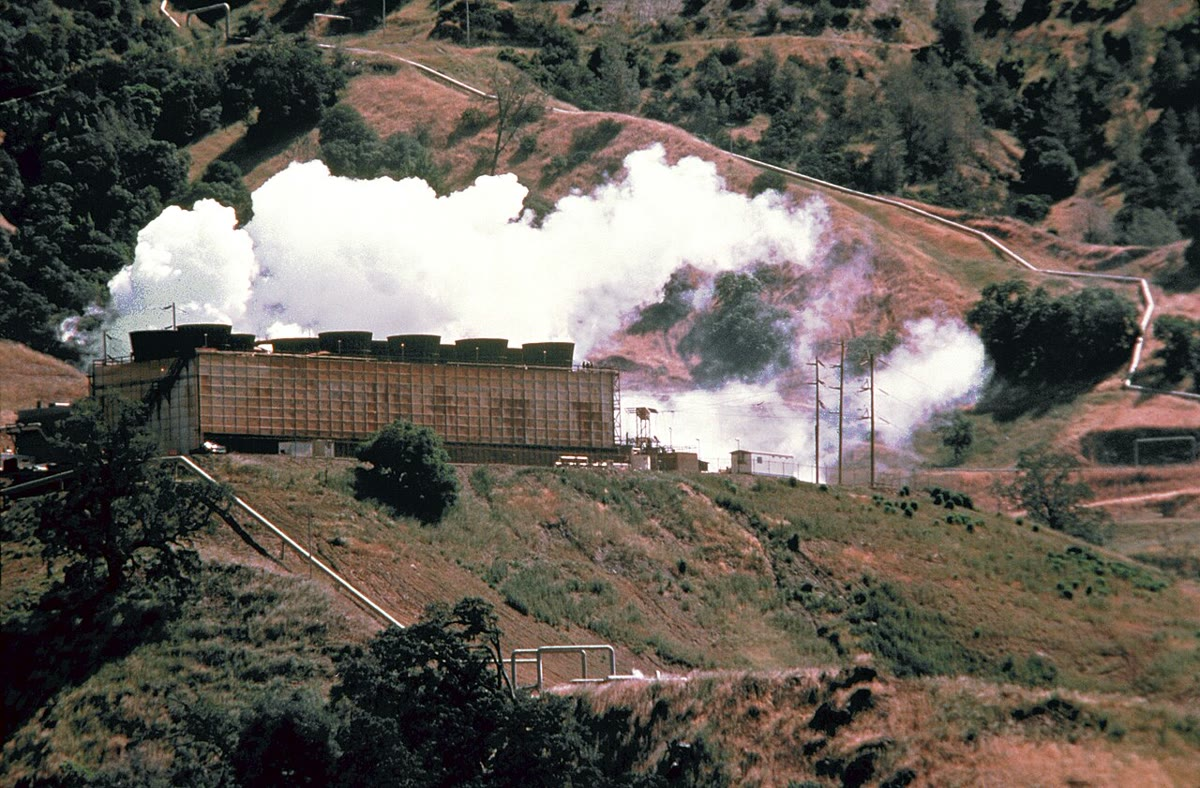
\includegraphics[width=\linewidth]{images/book4/b2-30-geyserville.jpg}
\end{minipage}
\par\smallskip{\small Links: een \omterm{def:b2:energy-geology:geothermal}{geothermisch systeem} met hoge enthalpie (schematisch, niet op schaal): water
dat aan de randen wordt aangevuld (blauw), wordt boven een intrusie verwarmd en stijgt door een gebroken reservoir
(rood) op naar een warmwaterbron; putten tappen het reservoir aan. Rechts: een geothermische centrale bij Geyserville,
Californië, in 1982, met stoomleidingen op de helling. Foto U.S. Department of Defense
(publiek domein).}
\end{omfigure}
% ledger: photo:b2-30-geyserville, usgs08g:egs

\begin{definition}[Geïnduceerde seismiciteit]\label{def:b2:energy-geology:induced}
\emph{Geïnduceerde seismiciteit}\index{geïnduceerde seismiciteit} is aardbevingsactiviteit veroorzaakt door menselijke
activiteiten die de spanning of de poriënvloeistofdruk in de korst veranderen, meestal de
injectie van vloeistof in de ondergrond.
\end{definition}

Het mechanisme is het criterium van Coulomb met poriënvloeistofdruk: een breuk glijdt wanneer de schuifspanning
$\mu(\sigma_n - p)$ bereikt, zodat een stijging van $p$ een breuk die al onder spanning staat naar bezwijken brengt
zonder enige verandering van de tektonische belasting. In de jaren 1960 veroorzaakte afvalvloeistof, geïnjecteerd in gebroken
precambrische sokkel onder het Rocky Mountain Arsenal bij Denver, op diepten van 3.7 tot
\qty{7.0}{km}, aardbevingen; ze bleven beperkt tot het deel van het reservoir waar de
druk met meer dan \qty{32}{bar} (\qty{3.2}{MPa}) was gestegen. De steile toename van de aardbevingen
in Oklahoma is toegeschreven aan de lozing van afvalwater: vier putten met een groot volume
zouden een vijfde van de seismiciteit van het centrum van de Verenigde Staten kunnen verklaren, en
aardbevingen op meer dan \qty{30}{km} afstand uitlokken. Het stimuleren van een EGS-reservoir verhoogt de poriëndruk op
dezelfde manier, met opzet.
% ledger: hb81:denver, keranen:oklahoma, usgs08g:egs

\section{Uranium}\label{sec:b2:energy-geology:uranium}

Twee \omterm{def:b2:ore-deposits:types}{ertsafzettingstypen} illustreren hoe uranium wordt geconcentreerd: het ene bij een oude discordantie, het
andere in zandsteen.

\begin{definition}[Discordantiegebonden uraniumafzetting en roll-front-uraniumafzetting]\label{def:b2:energy-geology:uranium}
Een \emph{discordantiegebonden uraniumafzetting}\index{discordantiegebonden uraniumafzetting} is een lichaam
van pekblende en uraniniet dat spleten en breccies opvult in gemetamorfoseerde koolstofhoudende pelieten en
in de kwartsarenieten erboven, onder, boven of over een discordantie tussen gesteenten uit het Vroeg- en
\omterm{def:b2:precambrian-earth:eons}{Midden-Proterozoïcum} in een \omterm{def:b2:basins-compared:types}{intracratonisch bekken}. Een \emph{roll-front-uraniumafzetting}\index{roll-front-uraniumafzetting}
is een sikkelvormig lichaam van uraniummineralen dat de gelaagdheid doorsnijdt van een
veldspaatrijke of tufhoudende zandsteen op de grens tussen geoxideerde en gereduceerde grond, waar
uranium werd afgezet in een plaatselijk reducerend milieu, tussen pyriet.
\end{definition}

De discordantieafzettingen zitten in gesteenten van 1800 tot \qty{1200}{\Ma}, de gemetamorfoseerde
pelieten onder de discordantie en de niet-gemetamorfoseerde zandstenen erboven; hun gastgesteenten zijn gechloritiseerd, en de grafietschisten die
veel ervan begeleiden, zijn sterke elektrische geleiders, een doelwit voor elektromagnetische metingen. Key
Lake, Cluff Lake en Rabbit Lake in Saskatchewan en Jabiluka en Ranger in het noorden van Australië zijn
voorbeelden. De roll-fronts zijn jonger, meestal tertiair: in zandstenen gevoed door felsische vulkanische as of
graniet liggen geoxideerde ijzermineralen hellingopwaarts van het front en gereduceerde hellingafwaarts, zoals in de bekkens
van Wyoming en de Golfkust van Texas.
% ledger: b1693:unconformity, b1693:sandstone

\begin{proposition}[Uranium-235 in het verleden]\label{prop:b2:energy-geology:u235}
Zij $r_0$ de huidige atomaire verhouding $^{235}$U/$^{238}$U en $\lambda_5$, $\lambda_8$ de
vervalconstanten van de twee isotopen. Een tijd $t$ geleden was de verhouding
\begin{equation}
r(t) = r_0\,e^{(\lambda_5 - \lambda_8)\,t} ,
\label{eq:b2:energy-geology:u235}
\end{equation}
en vormde $^{235}$U een fractie $r/(1 + r)$ van de uraniumatomen, als het spoor
$^{234}$U wordt verwaarloosd.
\end{proposition}

\begin{proof}
Elke isotoop vervalt exponentieel: $N_5(\text{nu}) = N_5(t)\,e^{-\lambda_5 t}$ en $N_8(\text{nu})
= N_8(t)\,e^{-\lambda_8 t}$. Delen geeft $r_0 = r(t)\,e^{-(\lambda_5 - \lambda_8)t}$.
\end{proof}

Met $\lambda_5 = \qty{9.8485e-10}{yr^{-1}}$, $\lambda_8 = \qty{1.55125e-10}{yr^{-1}}$ en de huidige
abundanties \qty{0.7204}{\percent} en \qty{99.2742}{\percent} is $r_0 = 0.0072567$; \qty{2.0}{\Ga}
geleden was $r = 0.0381$ en bevatte natuurlijk uranium \qty{3.67}{\percent} $^{235}$U, vijf keer het huidige
aandeel.
% ledger: amherst:constants, iaea:isotopes
% values: r 0.038144, 3.6743 % (calc/ch30.py)

\begin{history}[Een reactor van twee miljard jaar oud]
In 1972 vonden Franse wetenschappers bij metingen aan uraniumerts kleine maar significante tekorten aan
$^{235}$U, die ze herleidden tot de Oklo-mijn in Gabon. Daar bevatten lenzen gesteente tot
\qty{65}{\percent} uranium met soms maar de helft van het normale aandeel $^{235}$U, en neodymium
dat verarmd was in zijn primordiale isotoop $^{142}$Nd maar verrijkt in de isotopen 143 tot 150 die splijting
oplevert: er waren ongeveer twee miljard jaar geleden kettingreacties in het erts verlopen, bij ongeveer \qty{300}{bar}
en 400 tot \qty{500}{\celsius}. Er zijn zestien zulke natuurlijke reactoren bekend in Oklo en het nabije
Bangombé, de enige twee afzettingen ter wereld waar ze zijn gevonden; organisch materiaal had geholpen
het uranium te concentreren, en het uraniumoxide heeft sindsdien het grootste deel van de actiniden en van de
niet-vluchtige splijtingsproducten op hun plaats gehouden.
\end{history}
% ledger: oklo:curtis, oklo:cowan, oklo:gl96, oklo:nagy

\section{Geologische opslag van koolstofdioxide}\label{sec:b2:energy-geology:ccs}

\begin{definition}[Geologische opslag van \ce{CO2}, vangmechanismen, opslagefficiëntiefactor]\label{def:b2:energy-geology:ccs}
\emph{Geologische opslag van \ce{CO2}}\index{geologische opslag van CO$_2$} is de injectie van
koolstofdioxide in poreuze gesteenteformaties diep onder de grond, uitgeputte olie- en gasreservoirs, diepe zoute
formaties of steenkoollagen, om het daar lang vast te houden. De
\emph{vangmechanismen van \ce{CO2}}\index{vangmechanismen van CO$_2$} die het vasthouden, zijn structurele (en stratigrafische)
vangst onder een afdekgesteente; residuele vangst, als een onbeweeglijke fase die door capillaire krachten in de poriën wordt vastgehouden;
oplosvangst, door oplossing in het formatiewater; minerale vangst, door reactie
met mineralen tot carbonaten; en, in steenkool en schalie, adsorptie aan organisch materiaal. De
\emph{opslagefficiëntiefactor}\index{opslagefficiëntiefactor} $E$ van een formatie is de fractie van haar poriënvolume die de geïnjecteerde
\ce{CO2} naar verwachting kan vullen.
\end{definition}
% ledger: srccs:retention, netl08:saline

Koolstofdioxide is een gas aan het oppervlak, maar zijn kritieke punt ligt bij \qty{31.0}{\celsius} en
\qty{7.38}{MPa}. Langs een geotherm van \qty{25}{\celsius\per\km} vanaf \qty{15}{\celsius} onder
hydrostatische druk passeert de temperatuur de kritieke waarde op \qty{641}{m} en de druk op
\qty{742}{m}; de dichtheid van zuivere \ce{CO2} springt van \qty{234}{kg.m^{-3}} op \qty{700}{m} naar
\qty{583}{kg.m^{-3}} op \qty{900}{m}, en vlakt daarna af rond 670 tot \qty{700}{kg.m^{-3}} onder
\qty{1.5}{km}. Een ton neemt \qty{534}{m^3} in aan het oppervlak en \qty{1.6}{m^3} op \qty{1000}{m},
330 keer minder; daarom beschouwen beoordelingen van de opslag alleen formaties dieper dan
\qty{800}{m}.
% ledger: nist:co2-critical, data:b4-co2-density, srccs:density, netl08:saline
% values: z_tc 641.2 m, z_pc 742.2 m; volume ratio 331.9 (figdata co2_density.py numbers)

\begin{omfigure}
\centering
\begin{minipage}[b]{0.49\linewidth}\centering
\begin{tikzpicture}
\begin{axis}[omrecord, width=0.95\linewidth, height=5.2cm, xmin=0, xmax=750, ymin=0, ymax=3,
  y dir=reverse, xlabel={dichtheid van \ce{CO2} (\unit{kg.m^{-3}})}, ylabel={diepte (km)},
  tick label style={font=\scriptsize}, label style={font=\small}]
% computed in figdata/bachelor-2/co2_density.py part profile; ledger: data:b4-co2-density
\addplot[black!45, densely dashed] coordinates {(0,0.742) (750,0.742)};
\node[font=\tiny, text=black!60, anchor=south east] at (axis cs:745,0.73) {kritieke druk};
\addplot[omDef, line width=1.1pt, mark=*, mark size=0.9pt] table[x=rho, y expr=\thisrow{depth_m}/1000] {figdata/out/bachelor-2-co2_density-profile.dat};
\end{axis}
\end{tikzpicture}
\end{minipage}\hfill
\begin{minipage}[b]{0.49\linewidth}\centering
\begin{tikzpicture}
\begin{axis}[width=0.95\linewidth, height=5.2cm, xmin=0, xmax=4, ymin=0, ymax=100,
  axis x line=bottom, axis y line=left, axis line style={-}, axis on top,
  xlabel={tijd na injectie (jaar)}, ylabel={aandeel opgeslagen \ce{CO2}},
  xtick={0,1,2,3,4}, xticklabels={1,10,100,1000,$10^4$}, ytick=\empty,
  tick label style={font=\scriptsize}, label style={font=\small}]
% schematic, after IPCC SRCCS (2005) Figure 5.9; ledger: srccs:trapping
% bands from the bottom: mineral, solubility, residual, structural (cumulative tops 0/0/1/5/15,
% 2/8/21/40/60, 10/30/56/80/90, 100)
\fill[omLithLime!60!black] (axis cs:0,0) -- (axis cs:1,0) -- (axis cs:2,1) -- (axis cs:3,5) -- (axis cs:4,15) -- (axis cs:4,0) -- cycle;
\fill[omDef!40] (axis cs:0,0) -- (axis cs:1,0) -- (axis cs:2,1) -- (axis cs:3,5) -- (axis cs:4,15) -- (axis cs:4,60) -- (axis cs:3,40) -- (axis cs:2,21) -- (axis cs:1,8) -- (axis cs:0,2) -- cycle;
\fill[omProp!40] (axis cs:0,2) -- (axis cs:1,8) -- (axis cs:2,21) -- (axis cs:3,40) -- (axis cs:4,60) -- (axis cs:4,90) -- (axis cs:3,80) -- (axis cs:2,56) -- (axis cs:1,30) -- (axis cs:0,10) -- cycle;
\fill[black!15] (axis cs:0,10) -- (axis cs:1,30) -- (axis cs:2,56) -- (axis cs:3,80) -- (axis cs:4,90) -- (axis cs:4,100) -- (axis cs:0,100) -- cycle;
\node[font=\scriptsize] at (axis cs:1.1,72) {structureel};
\node[font=\scriptsize] at (axis cs:2.1,38) {residueel};
\node[font=\scriptsize] at (axis cs:3.1,22) {opgelost};
\node[font=\scriptsize, text=white, anchor=south east] at (axis cs:3.98,0.5) {mineraal};
\end{axis}
\end{tikzpicture}
\end{minipage}
\par\smallskip{\small Links: dichtheid van zuivere \ce{CO2} met de diepte langs een geotherm van
\qty{25}{\celsius\per\km} vanaf \qty{15}{\celsius}, onder hydrostatische druk. Gegevens: NIST Chemistry
WebBook (toestandsvergelijking van Span--Wagner), bij de omstandigheden van het IPCC Special Report on Carbon
Dioxide Capture and Storage (2005). Rechts: hoe de vangmechanismen de opgeslagen \ce{CO2} onderling verdelen
in de tijd (schematisch, naar hetzelfde rapport): de vangst door het afdekgesteente maakt plaats voor de residuele,
opgeloste en minerale vormen, die minder beweeglijk zijn.}
\end{omfigure}

\begin{proposition}[Opslagcapaciteit van een formatie]\label{prop:b2:energy-geology:capacity}
Een formatie met oppervlakte $A$, dikte $h$ en porositeit $\phi$, waarin \ce{CO2} de dichtheid $\rho$ heeft
en de \omterm{def:b2:energy-geology:ccs}{opslagefficiëntiefactor} $E$ is, kan de massa
\begin{equation}
M = A\,h\,\phi\,\rho\,E .
\label{eq:b2:energy-geology:capacity}
\end{equation}
opslaan. Voor een uitgeput olieveld dat een volume $N_p$ in tankcondities heeft geproduceerd, geeft het vervangen van de geproduceerde olie,
volume voor volume, $M = \rho\,N_p\,B_o$.
\end{proposition}

\begin{proof}
Het poriënvolume is $Ah\phi$, waarvan de \ce{CO2} een fractie $E$ vult, met dichtheid $\rho$. In het
olieveld nam de geproduceerde olie $N_pB_o$ in het reservoir in, het volume dat de \ce{CO2} overneemt.
\end{proof}

Voor diepe zoute formaties geven simulaties een $E$ tussen 1 en \qty{4}{\percent} van het poriënvolume
over een betrouwbaarheidsbereik van 15 tot 85 procent, met een mediaan rond \qty{2}{\percent}: het grootste deel van de
poriënruimte wordt nooit bereikt, of houdt zijn water. Een formatie van \qty{1000}{km^2}, \qty{50}{m} dik en met
porositeit 0.20 op \qty{2000}{m} ($\rho = \qty{686}{kg.m^{-3}}$) slaat \qty{137}{Mt} op bij $E =
\qty{2}{\percent}$.
% ledger: netl08:saline, data:b4-co2-density
% values: 1e9*50*0.2*686*0.02 = 1.372e11 kg (calc/ch30.py)

Eenmaal geïnjecteerd stijgt de \ce{CO2} onder het afdekgesteente en spreidt ze zich uit. Achter de migrerende pluim houden capillaire
krachten residuele verzadigingen vast die 15 tot \qty{25}{\percent} van de poriënruimte kunnen bereiken;
oplossing neemt 20 tot \qty{60}{kg} \ce{CO2} op per kubieke meter formatiewater, en in
langzaam stromende formaties lost tot \qty{30}{\percent} van de geïnjecteerde \ce{CO2} op binnen enkele tientallen
jaren. Oplosvangst overheerst over tientallen tot honderden jaren, ionische vormen over honderden tot
duizenden, minerale vangst over duizenden tot miljoenen: reacties met carbonaatmineralen duren dagen,
met silicaten honderden tot duizenden jaren. De opslag wordt veiliger naarmate ze ouder wordt, en op
goed gekozen en goed beheerde locaties werd het waarschijnlijk geacht dat \qty{99}{\percent} of meer van de \ce{CO2} over
1000 jaar wordt vastgehouden.
% ledger: srccs:trapping, srccs:retention

\begin{dated}{2005}
In Sleipner, in de Noordzee ongeveer \qty{250}{km} uit de kust van Noorwegen, wordt de \ce{CO2} die wordt afgescheiden uit het
aardgas van het veld, ongeveer \qty{9}{\percent} ervan, sinds oktober 1996 geïnjecteerd in
de Utsira-formatie, een ongeconsolideerde zoute zandsteen 800 tot \qty{1000}{m} onder de zeebodem,
met ongeveer \qty{1}{Mt} per jaar. Begin 2005 was meer dan \qty{7}{Mt} opgeslagen, van de \qty{20}{Mt}
die over de levensduur van het project gepland was. Herhaalde seismische opnamen brengen de pluim in beeld, waarvan de voetafdruk toen
ongeveer \qty{5}{km^2} was, en tonen dat het afdekgesteente erboven hem afsluit.
\end{dated}
% ledger: srccs:sleipner

\begin{inthefield}[Een put lezen terwijl hij wordt geboord]
\centering
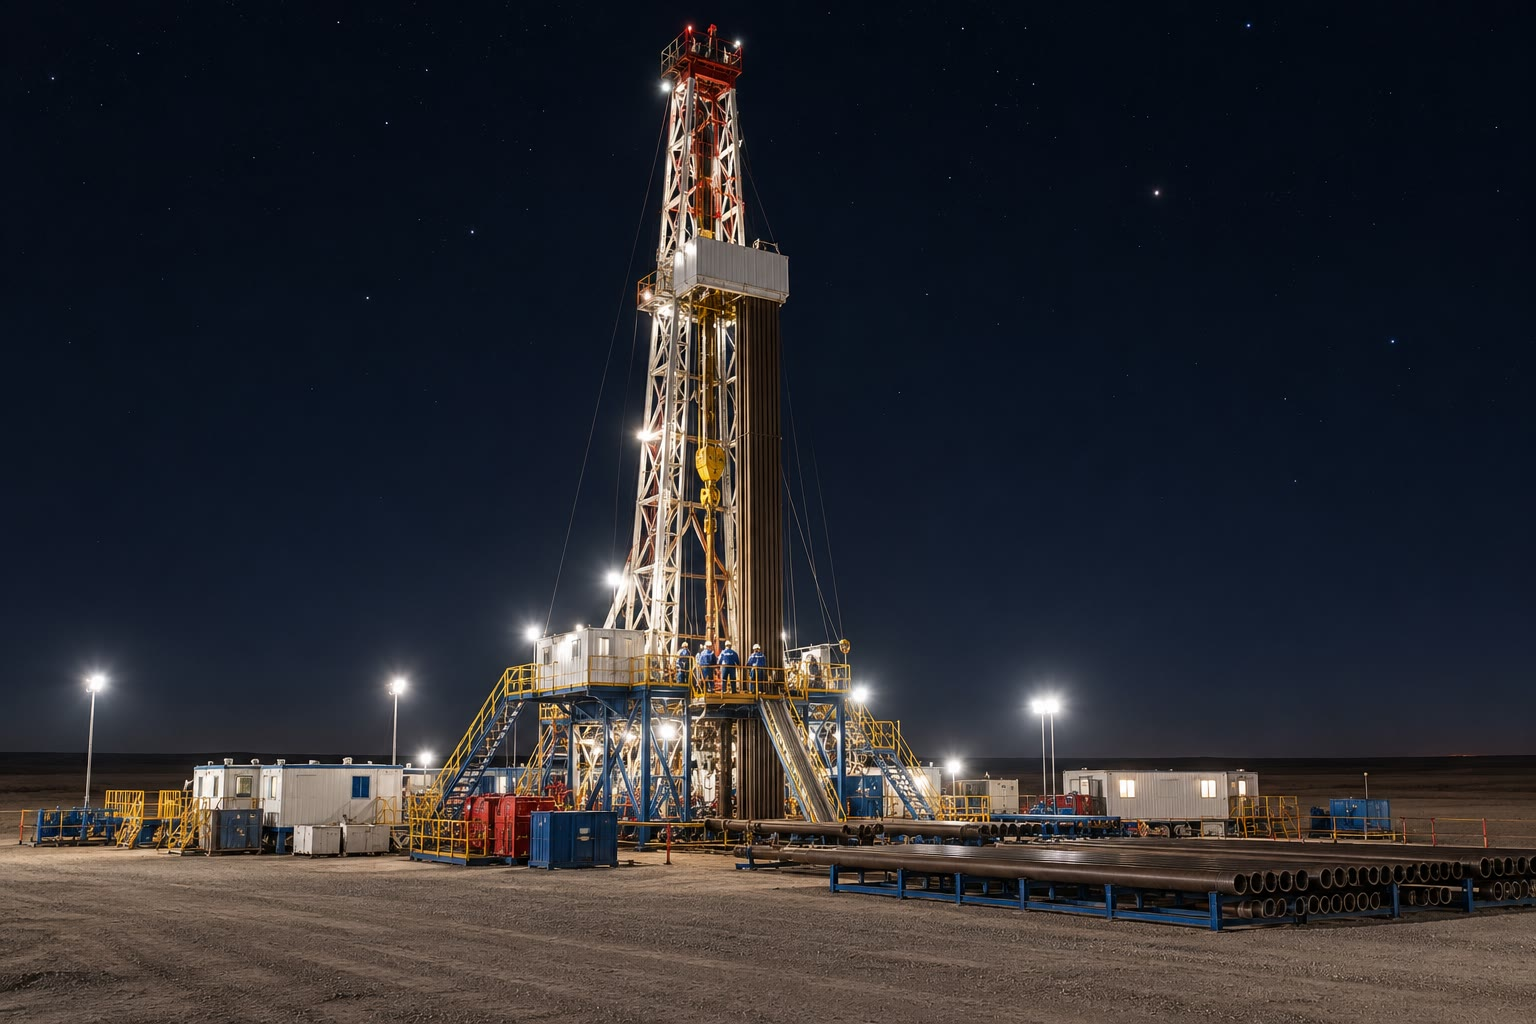
\includegraphics[width=0.56\linewidth]{images/book4/ai/b2-rig-night.jpg}
\par\smallskip{\small Een booreiland op het land bij nacht (door AI gegenereerde illustratie).}
\par\medskip\raggedright
Wanneer een sectie van een put klaar is, laten geofysici instrumenten aan een kabel zakken en registreren ze tegen de
diepte de eigenschappen van de gesteenten rond het gat. Eén instrument registreert hun natuurlijke radioactiviteit, laag in
zandsteen en hoger in schalie; een ander hun bulkdichtheid, waaruit de porositeit volgt als
(korreldichtheid $-$ bulkdichtheid)/(korreldichtheid $-$ vloeistofdichtheid), met \qty{2.65}{g/cm^3} voor
kwartskorrels en ongeveer \qty{1}{g/cm^3} voor het water. Samen gelezen geven deze boorgatmetingen de
netto reservoirdikte en de porositeit die in de volumetrische formules van dit hoofdstuk worden gebruikt.
\end{inthefield}
% ledger: keys:gamma, keys:density-porosity

\section*{Oefeningen}\label{sec:b2:energy-geology:exercises}

Gegevens voor de oefeningen, tenzij anders vermeld: $R = \qty{8.314}{J.mol^{-1}.K^{-1}}$; één miljoen
jaar is \qty{3.156e13}{s}; Green River-kerogeen $A = \qty{9.21e13}{s^{-1}}$, $E/R = \qty{26800}{K}$;
atoommassa's C 12.011, H 1.008, O 15.999; dichtheid van \ce{CO2} langs het profiel van de figuur:
\qty{1.872}{kg.m^{-3}} aan het oppervlak, 583 op \qty{900}{m}, 621 op \qty{1000}{m}, 686 op
\qty{2000}{m}. Rond af op drie beduidende cijfers.
% ledger: codata:R, fp14:gr-daem, data:b4-co2-density

\begin{exercise}[$\star$]\label{exo:b2:energy-geology:1}
(a) Vier onrijpe kerogenen hebben een atomaire H/C van 1.58, 0.95, 1.24 en 1.12. Ken elk een type toe en zeg
welke vooral gas zou leveren. (b) Controleer de verhoudingen H/C en O/C van de formule
C$_{100}$H$_{150}$N$_3$O$_8$S. (c) Bepaal ze uit de massasamenstelling C \qty{77.4}{\percent}, H
\qty{9.8}{\percent}, O \qty{8.2}{\percent}.
\end{exercise}

\begin{exercise}[$\star$]\label{exo:b2:energy-geology:2}
(a) Vijf monsters van een brongesteente van type~II hebben $R_o$ = 0.45, 0.68, 1.1, 1.6 en \qty{2.5}{\percent}.
Beschrijf de toestand van elk wat olie en gas betreft. (b) Levert een kerogeen van type~III bij $R_o =
\qty{0.68}{\percent}$ methaan? (c) Welke omgezette fractie $F$ van Easy\%Ro komt overeen met
$R_o = 0.6$ en \qty{1.3}{\percent}?
\end{exercise}

\begin{exercise}[$\star$]\label{exo:b2:energy-geology:3}
Een val beslaat \qty{6}{km^2}; het reservoir heeft \qty{25}{m} netto dikte, porositeit 0.18 en
waterverzadiging 0.30, en $B_o = 1.25$. (a) Bepaal het olievolume in het reservoir en de STOIIP. (b) Bepaal
het geproduceerde volume voor \omterm{def:b2:energy-geology:volumetrics}{winningsfactoren} van 0.30 en 0.40.
\end{exercise}

\begin{exercise}[$\star$]\label{exo:b2:energy-geology:4}
Een zandsteenaquifer van \qty{200}{m} dik onder \qty{10}{km^2} heeft een temperatuur van \qty{75}{\celsius}. (a) Bepaal de
\omterm{def:b2:energy-geology:geothermal}{aanwezige warmte} boven \qty{15}{\celsius}, met $C = \qty{2.5}{MJ.m^{-3}.K^{-1}}$. (b) Tot welke
enthalpieklasse behoort hij? (c) Bepaal het gemiddelde thermische vermogen over 30 jaar voor $R_g = 0.25$.
\end{exercise}

\begin{exercise}[$\star\star$]\label{exo:b2:energy-geology:5}
(a) Bepaal de activeringsenergie waarbij een Arrhenius-snelheid verdubbelt tussen 100 en
\qty{110}{\celsius}. (b) Met welke factor groeit de snelheid van de Green River-reactie over hetzelfde
interval? (c) Welke van de twee regels geeft meer gewicht aan de tijd die een gesteente bij lage temperatuur doorbracht,
en wat betekent dit voor een TTI die voor een brongesteente van type~I wordt berekend?
\end{exercise}

\begin{exercise}[$\star\star$]\label{exo:b2:energy-geology:6}
(a) Toon uit \eqref{eq:b2:energy-geology:maturation} aan dat de temperatuur van halve omzetting voldoet aan
$T = (E/R)\big/\ln\bigl[A T^2/(\beta\,(E/R)\ln 2)\bigr]$, en los dit iteratief op voor het Green
River-kerogeen verhit met \qty{1}{\celsius\per\Myr} en met \qty{10}{K} per minuut. (b) Vergelijk het
verschil met de schatting $(RT^2/E)\ln(\beta_2/\beta_1)$ genomen bij de laagste temperatuur, en
verklaar de afwijking.
\end{exercise}

\begin{exercise}[$\star\star$]\label{exo:b2:energy-geology:7}
Gebruik \eqref{eq:b2:energy-geology:u235} en de gegevens van de tekst: (a) bepaal het aandeel $^{235}$U in
natuurlijk uranium \qty{2.0}{\Ga} en \qty{1.8}{\Ga} geleden; (b) wanneer was het \qty{3.00}{\percent}?
(c) Erts van Oklo bevat soms maar de helft van het huidige normale aandeel $^{235}$U. Verwaarloos het $^{238}$U
dat werd verbruikt: welke fractie van het $^{235}$U dat ten tijde van de reacties aanwezig was, werd gespleten, en
waarom verandert het latere verval het antwoord niet?
\end{exercise}

\begin{exercise}[$\star\star$]\label{exo:b2:energy-geology:8}
(a) Bepaal het volume van \qty{1}{Mt} \ce{CO2} aan het oppervlak, op \qty{1000}{m} en op
\qty{2000}{m}. (b) In Sleipner was tegen 2005 meer dan \qty{7}{Mt} geïnjecteerd, op ongeveer
\qty{900}{m}, in een pluim met een voetafdruk van \qty{5}{km^2}. Neem een porositeit van 0.35 en een
\ce{CO2}-verzadiging van 0.30 in de pluim, en bepaal het volume gesteente dat hij inneemt en zijn gemiddelde dikte.
\end{exercise}

\begin{exercise}[$\star\star$]\label{exo:b2:energy-geology:9}
Een hoge-enthalpiereservoir meet $3 \times 2 \times \qty{1.5}{km}$ bij \qty{250}{\celsius}, met
$C = \qty{2.6}{MJ.m^{-3}.K^{-1}}$. (a) Bepaal de \omterm{def:b2:energy-geology:geothermal}{aanwezige warmte} boven \qty{15}{\celsius}. (b) Bepaal het
gemiddelde thermische vermogen over 30 jaar voor $R_g = 0.1$ en $0.25$. (c) Het veld beslaat \qty{6}{km^2};
bij 10 tot \qty{20}{MW} elektriciteit per vierkante kilometer, welke fractie van het thermische vermogen bij
$R_g = 0.1$ wordt elektriciteit?
\end{exercise}

\begin{exercise}[$\star\star\star$]\label{exo:b2:energy-geology:10}
Een breuk op ongeveer \qty{4}{km} draagt een normaalspanning van \qty{80}{MPa} en een schuifspanning van
\qty{22}{MPa}; de wrijvingscoëfficiënt is 0.6 en de poriëndruk is hydrostatisch,
\qty{39}{MPa}. (a) Is de breuk stabiel? Bepaal de stijging van de poriëndruk die haar tot bezwijken brengt, in
megapascal en in bar, en vergelijk met de drempel van Denver. (b) Hetzelfde als de schuifspanning
\qty{24}{MPa} is. (c) Leg uit waarom aardbevingen kilometers van een injectieput kunnen worden uitgelokt,
en jaren nadat de injectie begon.
\end{exercise}

\begin{exercise}[$\star\star\star$]\label{exo:b2:energy-geology:11}
(a) Toon uit de benadering in \eqref{eq:b2:energy-geology:maturation} aan dat bij een constante
verhittingssnelheid de omzettingsgraad stijgt van \qty{10}{\percent} tot \qty{90}{\percent} over een
temperatuurinterval $\Delta T \approx \bigl[\ln\ln 10 - \ln\ln(10/9)\bigr]\,RT^2/E$. (b) Bereken het
voor het Green River-kerogeen bij \qty{1}{\celsius\per\Myr}. (c) Vergelijk met de doorgetrokken curve van de
figuur en verklaar het verschil.
\end{exercise}

\begin{exercise}[$\star\star\star$]\label{exo:b2:energy-geology:12}
Sleipner moet \qty{20}{Mt} \ce{CO2} opslaan. (a) Bepaal het volume formatiewater dat nodig is om
alles op te lossen, bij 20 en bij \qty{60}{kg.m^{-3}}. (b) Bepaal het volume als vrije fase op
\qty{1000}{m}. (c) Bepaal met $E = \qty{2}{\percent}$ het vereiste poriënvolume van de formatie, en
de oppervlakte van een formatie van \qty{50}{m} dik met porositeit 0.30.
\end{exercise}
% ledger: srccs:trapping, srccs:sleipner, hb81:denver

\begin{problem}[{Weekendprobleem --- Eén bekken, twee toepassingen}]\label{pb:b2:energy-geology:1}
In een verzonnen bekken werd een brongesteente van type~I op \qty{120}{\Ma} aan het oppervlak afgezet.
Daarna hoopte sediment zich op met \qty{60}{m} per miljoen jaar tot \qty{70}{\Ma}, en met \qty{30}{m}
per miljoen jaar sindsdien. Het oppervlak heeft \qty{15}{\celsius} en de geotherm is constant,
\qty{25}{\celsius\per\km}. Het kerogeen heeft de Green River-kinetiek uit de tekst (één energie).
De keuken ervan, het rijpe deel van het brongesteente, beslaat \qty{400}{km^2}, is \qty{50}{m} dik,
heeft een dichtheid van \qty{2400}{kg.m^{-3}}, en kan bij volledige omzetting \qty{30}{kg} olie per ton gesteente
leveren; de olie heeft aan het oppervlak een dichtheid van \qty{850}{kg.m^{-3}}. De olie vult een val van
\qty{12}{km^2} waarvan het reservoir, gecentreerd op \qty{2000}{m}, een netto dikte van \qty{40}{m} heeft,
porositeit 0.22 en waterverzadiging 0.25, met $B_o = 1.30$. Gebruik de gegevens van de oefeningen; rond af op
drie beduidende cijfers.

\noindent\textbf{Deel I --- Begraving en de tijd--temperatuurindex.}
\begin{enumerate}
  \item Bepaal de diepte en de temperatuur van het brongesteente op \qty{70}{\Ma} en vandaag.
  \item Bepaal de verhittingssnelheid in elke fase.
  \item Bepaal de tijd die het in elk interval van \qty{10}{\celsius} doorbracht, van \qty{15}{\celsius} tot
        zijn huidige temperatuur.
  \item Bereken de huidige TTI (methode uit de tekst).
  \item Wanneer, bij welke temperatuur en op welke diepte passeerde het een TTI van 15?
  \item Hetzelfde voor 75 en 160.
  \item Levert het brongesteente volgens de TTI nog olie?
\end{enumerate}

\noindent\textbf{Deel II --- Omzetting volgens de kinetiek.}
\begin{enumerate}[resume]
  \item Bepaal de snelheidsconstante bij \qty{90}{\celsius} en toon aan dat minder dan \qty{0.2}{\percent} van
        het kerogeen vóór \qty{70}{\Ma} kan zijn omgezet.
  \item Bepaal met \eqref{eq:b2:energy-geology:maturation} en de verhittingssnelheid van de tweede fase
        de niet-omgezette fractie en de omzettingsgraad vandaag.
  \item Bepaal de temperatuur van halve omzetting bij deze verhittingssnelheid (oefening~\ref{exo:b2:energy-geology:6}).
  \item Wanneer werd die bereikt?
  \item Vergelijk met het tijdstip van maximale olievorming volgens de TTI, en verklaar het verschil.
  \item Zou een kerogeen van type~II met een lagere gemiddelde activeringsenergie eerder of later zijn omgezet?
\end{enumerate}

\noindent\textbf{Deel III --- Gevormde, aanwezige en winbare olie.}
\begin{enumerate}[resume]
  \item Bepaal, met een omzettingsgraad van 0.92, de massa olie die in de keuken is gevormd.
  \item Bepaal het volume ervan aan het oppervlak.
  \item Bepaal de STOIIP van de val.
  \item Welke fractie van de gevormde olie bevat de val? Houd \qty{1.56e9}{m^3} aan voor (15).
  \item Bepaal de geproduceerde olie voor een \omterm{def:b2:energy-geology:volumetrics}{winningsfactor} van 0.35.
  \item Waarom is de \omterm{def:b2:energy-geology:volumetrics}{winningsfactor} veel kleiner dan één, en wat zou het injecteren van \ce{CO2} veranderen?
\end{enumerate}

\noindent\textbf{Deel IV --- Het uitgeputte veld als opslag voor \ce{CO2}.}
\begin{enumerate}[resume]
  \item Bepaal de temperatuur en de hydrostatische druk van het reservoir. Is geïnjecteerde \ce{CO2}
        daar superkritisch? Lees de dichtheid ervan af op de figuur.
  \item Bepaal, met $N_p = \qty{2.13e7}{m^3}$, het reservoirvolume dat door de productie is vrijgekomen.
  \item Druk het uit als een \omterm{def:b2:energy-geology:ccs}{opslagefficiëntiefactor} van het poriënvolume van de val, en vergelijk met
        zoute formaties.
  \item Een zoute formatie onder het veld beslaat \qty{600}{km^2}, is \qty{80}{m} dik, heeft
        porositeit 0.20, met \ce{CO2} bij \qty{691}{kg.m^{-3}}. Bepaal haar capaciteit bij $E =
        \qty{2}{\percent}$.
  \item Hoeveel jaar injectie aan het tempo van Sleipner zou haar vullen?
  \item Bepaal, met $\rho = \qty{686}{kg.m^{-3}}$ en het vrijgekomen volume afgerond op \qty{2.77e7}{m^3},
        de opslagcapaciteit voor \ce{CO2} van het uitgeputte reservoir, in megaton.
\end{enumerate}
\end{problem}
% ledger: fp14:gr-daem, waples80:tti, hamm14:tti-table, netl08:oilgas, netl08:saline, data:b4-co2-density, nist:co2-critical, srccs:sleipner
